\documentclass[landscape,a4paper,10pt]{article}
\usepackage{tikz}
\usepackage{verbatim}
\usepackage[landscape,margin=15mm]{geometry}
\usetikzlibrary{shapes,arrows,fit,calc,positioning}
\begin{document}
File created by KisTA library

Author: F.Herrera

Institution: KTH (2012-2014, Jul), Univ. of Cantabria (from 2014, Sept.)

Rights reserved by the authors in the terms defined by the KisTA license.

KisTA library compilation date: Jul 12 2016 at 10:36:03.

Tracing Options used:
Style=Clustered, Compact; Baselines sep.=1; Max. t span=3; Scale:=0.750000; Landscape; Show sched. activity.
\\
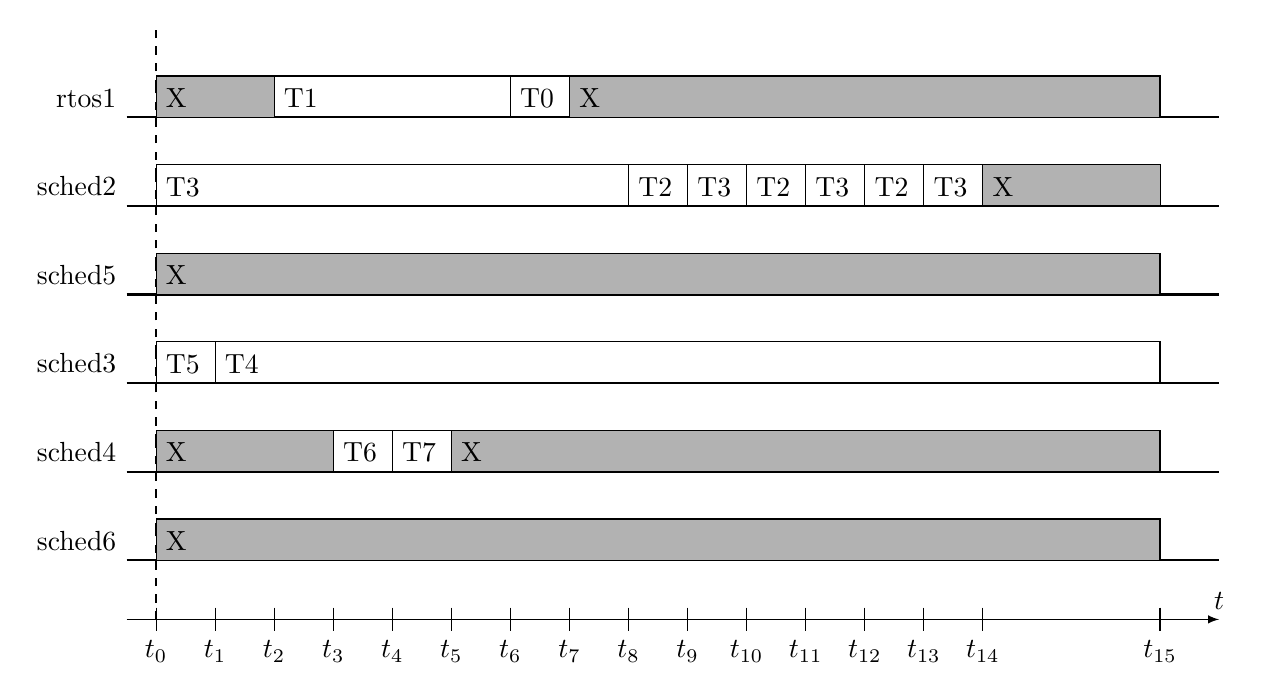
\begin{tikzpicture}[scale=0.750000]
% Draw time axis
% --------------
\draw [-latex](-0.5,0) coordinate(LEFTX)-- (0,0) coordinate (ORIG) -- (18,0) coordinate(RIGHTX) node[above]{$t$};

% Draw time axis divisions
% ------------------------
\draw[] (0,0.2) -- (0,-0.2)  node[below]{$t_{0}$};
\draw[] (1,0.2) -- (1,-0.2)  node[below]{$t_{1}$};
\draw[] (2,0.2) -- (2,-0.2)  node[below]{$t_{2}$};
\draw[] (3,0.2) -- (3,-0.2)  node[below]{$t_{3}$};
\draw[] (4,0.2) -- (4,-0.2)  node[below]{$t_{4}$};
\draw[] (5,0.2) -- (5,-0.2)  node[below]{$t_{5}$};
\draw[] (6,0.2) -- (6,-0.2)  node[below]{$t_{6}$};
\draw[] (7,0.2) -- (7,-0.2)  node[below]{$t_{7}$};
\draw[] (8,0.2) -- (8,-0.2)  node[below]{$t_{8}$};
\draw[] (9,0.2) -- (9,-0.2)  node[below]{$t_{9}$};
\draw[] (10,0.2) -- (10,-0.2)  node[below]{$t_{10}$};
\draw[] (11,0.2) -- (11,-0.2)  node[below]{$t_{11}$};
\draw[] (12,0.2) -- (12,-0.2)  node[below]{$t_{12}$};
\draw[] (13,0.2) -- (13,-0.2)  node[below]{$t_{13}$};
\draw[] (14,0.2) -- (14,-0.2)  node[below]{$t_{14}$};
\draw[] (17,0.2) -- (17,-0.2)  node[below]{$t_{15}$};

% Draw y axis
% --------------
\draw [dashed,thick]  (ORIG) -- (0,1)coordinate(sched6e0)  -- ++(0,0.5) coordinate(CLUSTER_0_YTOP);

\draw [dashed,thick]  (CLUSTER_0_YTOP) -- ++(0,1) coordinate(sched4e0)  -- ++(0,0.5) coordinate(CLUSTER_1_YTOP);

\draw [dashed,thick]  (CLUSTER_1_YTOP) -- ++(0,1) coordinate(sched3e0)  -- ++(0,0.5) coordinate(CLUSTER_2_YTOP);

\draw [dashed,thick]  (CLUSTER_2_YTOP) -- ++(0,1) coordinate(sched5e0)  -- ++(0,0.5) coordinate(CLUSTER_3_YTOP);

\draw [dashed,thick]  (CLUSTER_3_YTOP) -- ++(0,1) coordinate(sched2e0)  -- ++(0,0.5) coordinate(CLUSTER_4_YTOP);

\draw [dashed,thick]  (CLUSTER_4_YTOP) -- ++(0,1) coordinate(rtos1e0)  -- ++(0,0.5) coordinate(CLUSTER_5_YTOP);

\draw [dashed,thick] (CLUSTER_5_YTOP) -- ++(0,1) coordinate(YTOP);

% Draw baselines
% --------------
\draw [thick] (LEFTX|-sched6e0) node[above left]{sched6} -- (sched6e0-|RIGHTX);

\draw [thick] (LEFTX|-sched4e0) node[above left]{sched4} -- (sched4e0-|RIGHTX);

\draw [thick] (LEFTX|-sched3e0) node[above left]{sched3} -- (sched3e0-|RIGHTX);

\draw [thick] (LEFTX|-sched5e0) node[above left]{sched5} -- (sched5e0-|RIGHTX);

\draw [thick] (LEFTX|-sched2e0) node[above left]{sched2} -- (sched2e0-|RIGHTX);

\draw [thick] (LEFTX|-rtos1e0) node[above left]{rtos1} -- (rtos1e0-|RIGHTX);

% Set event coordinates   
% ------------------------
\path (sched6e0) ++ (17,0) coordinate(sched6e15);
\path (sched4e0) ++ (3,0) coordinate(sched4e3) ++ (1,0) coordinate(sched4e4) ++ (1,0) coordinate(sched4e5) ++ (12,0) coordinate(sched4e15);
\path (sched3e0) ++ (1,0) coordinate(sched3e1) ++ (16,0) coordinate(sched3e15);
\path (sched5e0) ++ (17,0) coordinate(sched5e15);
\path (sched2e0) ++ (8,0) coordinate(sched2e8) ++ (1,0) coordinate(sched2e9) ++ (1,0) coordinate(sched2e10) ++ (1,0) coordinate(sched2e11) ++ (1,0) coordinate(sched2e12) ++ (1,0) coordinate(sched2e13) ++ (1,0) coordinate(sched2e14) ++ (3,0) coordinate(sched2e15);
\path (rtos1e0) ++ (2,0) coordinate(rtos1e2) ++ (4,0) coordinate(rtos1e6) ++ (1,0) coordinate(rtos1e7) ++ (10,0) coordinate(rtos1e15);

% Draw scheduler activity (relying on event coordinates) 
% -------------------------------------------------------
\begin{scope}[shift={(sched6e0)}]
\draw[fill=black!30] (0,0) rectangle (17,0.7);
\draw[] (0,0) node[rectangle, above right] {X};
\end{scope}
\begin{scope}[shift={(sched4e0)}]
\draw[fill=black!30] (0,0) rectangle (3,0.7);
\draw[] (0,0) node[rectangle, above right] {X};
\end{scope}
\begin{scope}[shift={(sched4e3)}]
\draw[] (0,0) rectangle (1,0.7);
\draw[] (0,0) node[rectangle, above right] {T6};
\end{scope}
\begin{scope}[shift={(sched4e4)}]
\draw[] (0,0) rectangle (1,0.7);
\draw[] (0,0) node[rectangle, above right] {T7};
\end{scope}
\begin{scope}[shift={(sched4e5)}]
\draw[fill=black!30] (0,0) rectangle (12,0.7);
\draw[] (0,0) node[rectangle, above right] {X};
\end{scope}
\begin{scope}[shift={(sched3e0)}]
\draw[] (0,0) rectangle (1,0.7);
\draw[] (0,0) node[rectangle, above right] {T5};
\end{scope}
\begin{scope}[shift={(sched3e1)}]
\draw[] (0,0) rectangle (16,0.7);
\draw[] (0,0) node[rectangle, above right] {T4};
\end{scope}
\begin{scope}[shift={(sched5e0)}]
\draw[fill=black!30] (0,0) rectangle (17,0.7);
\draw[] (0,0) node[rectangle, above right] {X};
\end{scope}
\begin{scope}[shift={(sched2e0)}]
\draw[] (0,0) rectangle (8,0.7);
\draw[] (0,0) node[rectangle, above right] {T3};
\end{scope}
\begin{scope}[shift={(sched2e8)}]
\draw[] (0,0) rectangle (1,0.7);
\draw[] (0,0) node[rectangle, above right] {T2};
\end{scope}
\begin{scope}[shift={(sched2e9)}]
\draw[] (0,0) rectangle (1,0.7);
\draw[] (0,0) node[rectangle, above right] {T3};
\end{scope}
\begin{scope}[shift={(sched2e10)}]
\draw[] (0,0) rectangle (1,0.7);
\draw[] (0,0) node[rectangle, above right] {T2};
\end{scope}
\begin{scope}[shift={(sched2e11)}]
\draw[] (0,0) rectangle (1,0.7);
\draw[] (0,0) node[rectangle, above right] {T3};
\end{scope}
\begin{scope}[shift={(sched2e12)}]
\draw[] (0,0) rectangle (1,0.7);
\draw[] (0,0) node[rectangle, above right] {T2};
\end{scope}
\begin{scope}[shift={(sched2e13)}]
\draw[] (0,0) rectangle (1,0.7);
\draw[] (0,0) node[rectangle, above right] {T3};
\end{scope}
\begin{scope}[shift={(sched2e14)}]
\draw[fill=black!30] (0,0) rectangle (3,0.7);
\draw[] (0,0) node[rectangle, above right] {X};
\end{scope}
\begin{scope}[shift={(rtos1e0)}]
\draw[fill=black!30] (0,0) rectangle (2,0.7);
\draw[] (0,0) node[rectangle, above right] {X};
\end{scope}
\begin{scope}[shift={(rtos1e2)}]
\draw[] (0,0) rectangle (4,0.7);
\draw[] (0,0) node[rectangle, above right] {T1};
\end{scope}
\begin{scope}[shift={(rtos1e6)}]
\draw[] (0,0) rectangle (1,0.7);
\draw[] (0,0) node[rectangle, above right] {T0};
\end{scope}
\begin{scope}[shift={(rtos1e7)}]
\draw[fill=black!30] (0,0) rectangle (10,0.7);
\draw[] (0,0) node[rectangle, above right] {X};
\end{scope}
\end{tikzpicture}

% Show Automatic Task Alias names 
% --------------------------------
\textbf{Task alias list (alias=task name):}\\
T7=T8 , 
T3=T4 , 
T5=T6 , 
T4=T5 , 
T2=T3 , 
T6=T7 , 
T1=T2 , 
T0=T1\\

% Show Time stamp values
% ---------------------
\textbf{Time Stamp values:}\\
$t_{0} = 9 ms; t_{1} = 9026799674 ps; t_{2} = 9030919348 ps; t_{3} = 9032042883 ps; t_{4} = 9036062883 ps; t_{5} = 9040062883 ps; t_{6} = 9074459348 ps; t_{7} = 9096759348 ps; t_{8} = 9155520 ns; t_{9} = 9235640 ns; t_{10} = 9932020 ns; t_{11} = 10012140 ns; t_{12} = 10703440 ns; t_{13} = 10783560 ns; t_{14} = 11475540 ns; t_{15} = 17650879674 ps;  \\
$

% Show Time span values
% ---------------------
\textbf{Time Span values:}\\
$t_{1} - t_{0} = 26799674 ps; t_{2} - t_{1} = 4119674 ps; t_{3} - t_{2} = 1123535 ps; t_{4} - t_{3} = 4020 ns; t_{5} - t_{4} = 4 us; t_{6} - t_{5} = 34396465 ps; t_{7} - t_{6} = 22300 ns; t_{8} - t_{7} = 58760652 ps; t_{9} - t_{8} = 80120 ns; t_{10} - t_{9} = 696380 ns; t_{11} - t_{10} = 80120 ns; t_{12} - t_{11} = 691300 ns; t_{13} - t_{12} = 80120 ns; t_{14} - t_{13} = 691980 ns; t_{15} - t_{14} = 6175339674 ps;  \\
$

\end{document}

